%%%%%%%Esempi di utili di possibili azioni 

%%Esempio pseudo algoritmo usando come env algorithm -> appare in listofalgorithms
\begin{algorithm}
    \caption{Nome algortimo}\label{algo:name}
    \begin{algorithmic}[1]
        \Require $\text{Input dell'algoritmo}$
        \Ensure $\text{Output dell'algortimo}$
        \State variabile $\gets$ assegnazione valore
        \State valore\_ritornato $\gets$ \textsc{Funzione}\textsc{Prova}(param1, param2)

        \For{\textit{element} in \textit{list}} 
            \State res $\gets$ \textsc{Do}\textsc{Something}(element)
        \EndFor

        \If{condizione1}
            \State do something

        \ElsIf{condizione2}
            \State do something else
        \Else
            \State \textbf{print} ``Hello World"
        \EndIf
    \end{algorithmic}
\end{algorithm}

%%Esempio importazione codice da file -> appare su listofalgorithms
\lstinputlisting[language=Python, caption=Didascalia., label=ls:codice]{code/randomized_search.py}

%%Esempio immagine
\begin{figure}
    \centering
    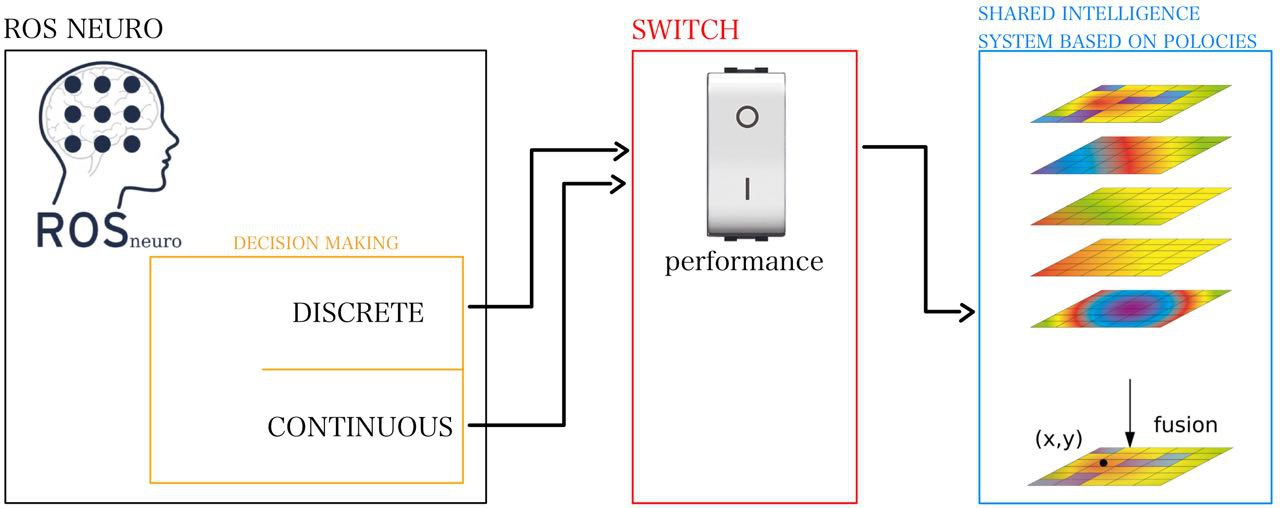
\includegraphics[scale=0.3]{images/Intro.jpg}
    \caption{Schematization on what I wanto to do}
    \label{fig:intro}
\end{figure}

%%Esempio citazione
\cite{5910562}

%%Esempio formula su più righe
\begin{equation}
    \begin{split}
        x(t) &= x_{0} + v_{0}t + \frac{1}{2}at^{2} \\ & =
		    x_{0} + v_{0}t + \frac{1}{2}\frac{F}{m}t^{2}
    \end{split}
\end{equation}

%%Per tabelle suggeriamo il sito: https://www.tablesgenerator.com/latex_tables